\documentclass[10pt,twocolumn,letterpaper]{article}

\usepackage{cvpr}
\usepackage{times}
\usepackage{epsfig}
\usepackage{graphicx}
\usepackage{amsmath}
\usepackage{amssymb}
\usepackage[margin=0.5in]{geometry}
\usepackage{pgfplots}
\usepackage{csvsimple}
\usepackage{xcolor}
\usepackage{multirow}
\usepackage{array}
\pgfplotsset{width=10cm, compat=1.9}
\usepackage[encapsulated]{CJK} 

% Include other packages here, before hyperref.

% If you comment hyperref and then uncomment it, you should delete
% egpaper.aux before re-running latex.  (Or just hit 'q' on the first latex
% run, let it finish, and you should be clear).
\usepackage[breaklinks=true,bookmarks=false]{hyperref}

% *** Uncomment this line for the final submission
\cvprfinalcopy{}

% *** Enter the CVPR Paper ID here
\def\cvprPaperID{****}
\def\httilde{\mbox{\tt\raisebox{-.5ex}{\symbol{126}}}}

% Pages are numbered in submission mode, and unnumbered in camera-ready
%\ifcvprfinal\pagestyle{empty}\fi
\setcounter{page}{1}
\begin{document}
\begin{CJK}{UTF8}{bkai}
   %%%%%%%%% TITLE
   \title{Contrastive Learning for Speech Enhancement}

   \author{郭品辰\\
      F14066127\\
      NCKU SNAME
      \and
      黃仁鴻\\
      P76094169\\
      NCKU CSIE}

   \maketitle

   \section{Introduction}

   許多與日常生活息息相關的任務都是仰賴語音作為資訊傳遞的媒介,像是電話通訊、語音辨識與助聽器等等。然而在現實環境中充滿著各種不可預期的噪音干擾,這嚴重影響了語音訊號技術的效能。因此,將這些雜訊去除的語音增強技術就成了對語音任務很重要的前置處理單元。

   而語音增強的問題就是不論在何種噪音環境,面對相同的語音,模型都能夠抽取出相同的特徵,進而利用與特徵來重構語音。這部分想法與近年流行自監督方法中的對比學習
   (Contrastive Learning) 不謀而合,對比學習希望相似樣本間的特徵編碼能越像越好,而不同樣本的特徵差異則是越大越好。

   我們認為,藉由 CL 的方法來學習語音特徵的潛在編碼,再利用此特徵編碼還原語音,應該會具備比一般深度學習的語音增強方法更高的通用性與泛化能力。因此,本次專題研究的主軸便是將對比學習應用於語音增強任務的可行性。
   \begin{figure}[t]
      \begin{center}
         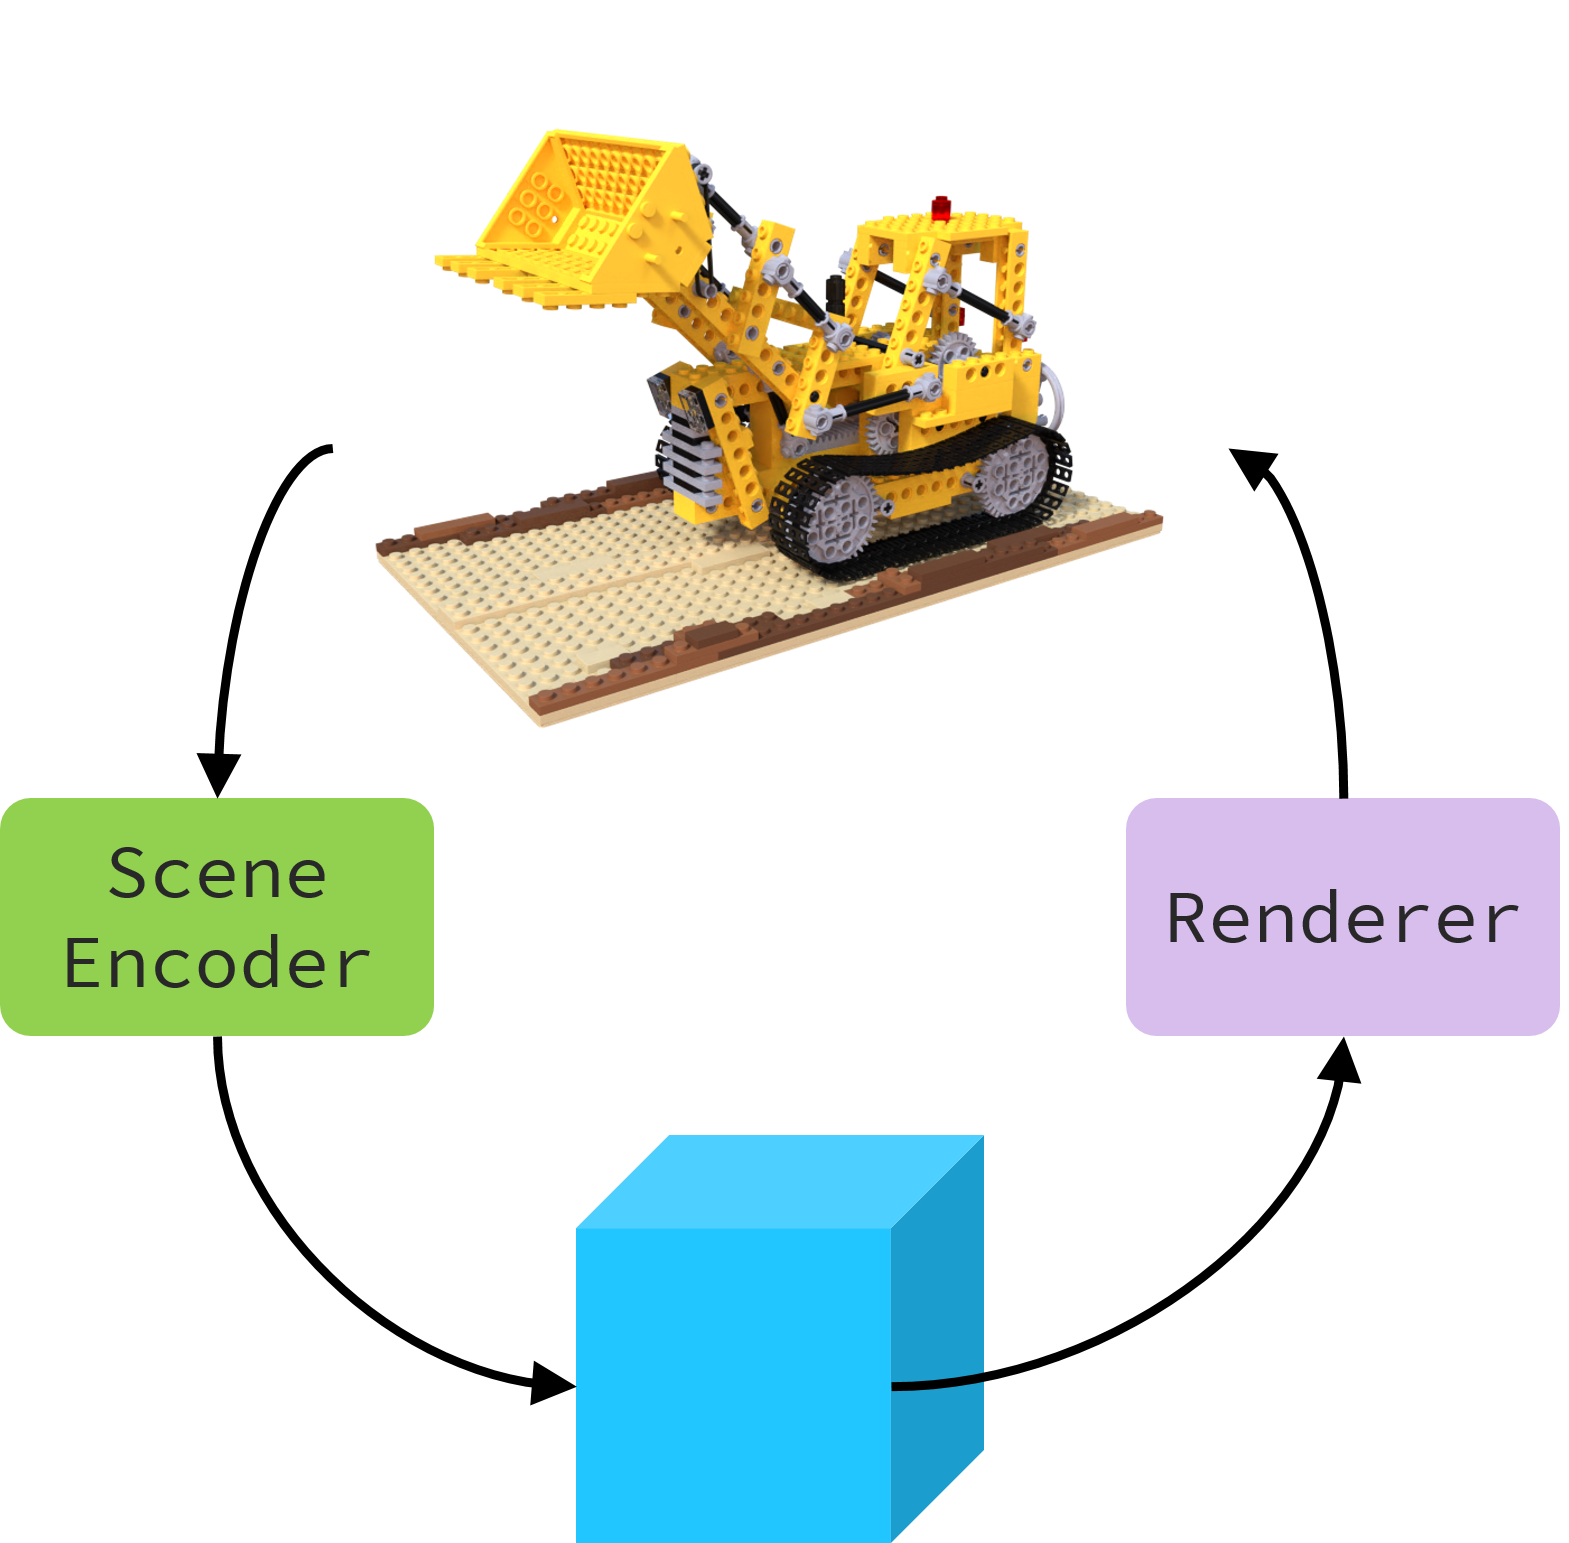
\includegraphics[width=1\linewidth]{img/auto-encoder.png}
      \end{center}
      \caption{語音增強使用的 Auto Encoder。期望模型能將受雜訊污染的語音還原成乾淨語音。\label{fig:auto-encode}}
   \end{figure}

   \begin{figure}[t]
      \begin{center}
         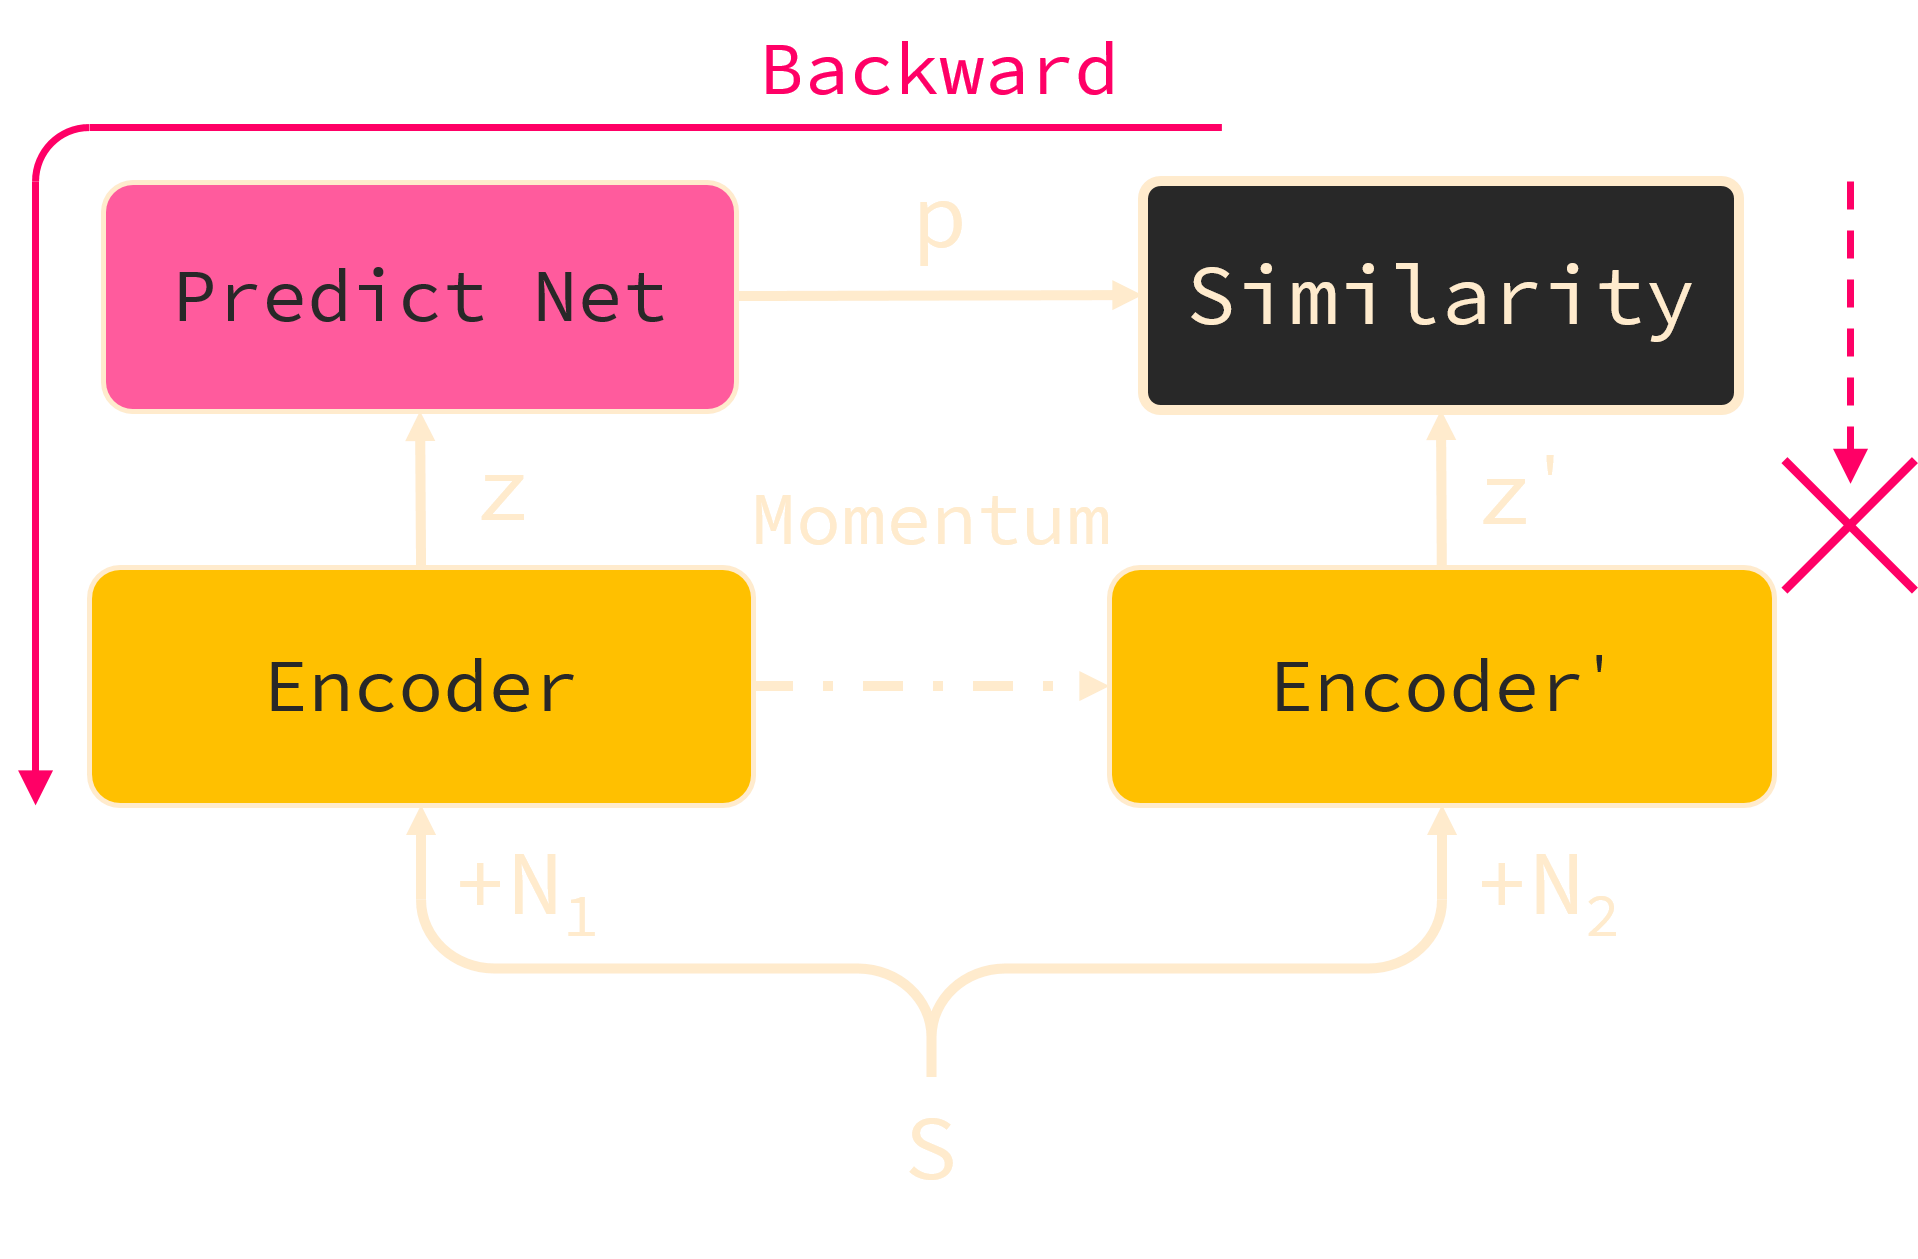
\includegraphics[width=1\linewidth]{img/BYOL.png}
      \end{center}
      \caption{BYOL 的算法架構。Encoder-PredictNet 會將 Encoder' 取出特徵做為目標,
         計算 L2 Loss 後更新 Encoder-PredictNet 的參數,
         Encoder' 則會把自身目前參數與更新後 Encoder 做加權平均當新參數。\label{fig:BYOL}}
   \end{figure}

   \begin{figure}[t]
      \begin{center}
         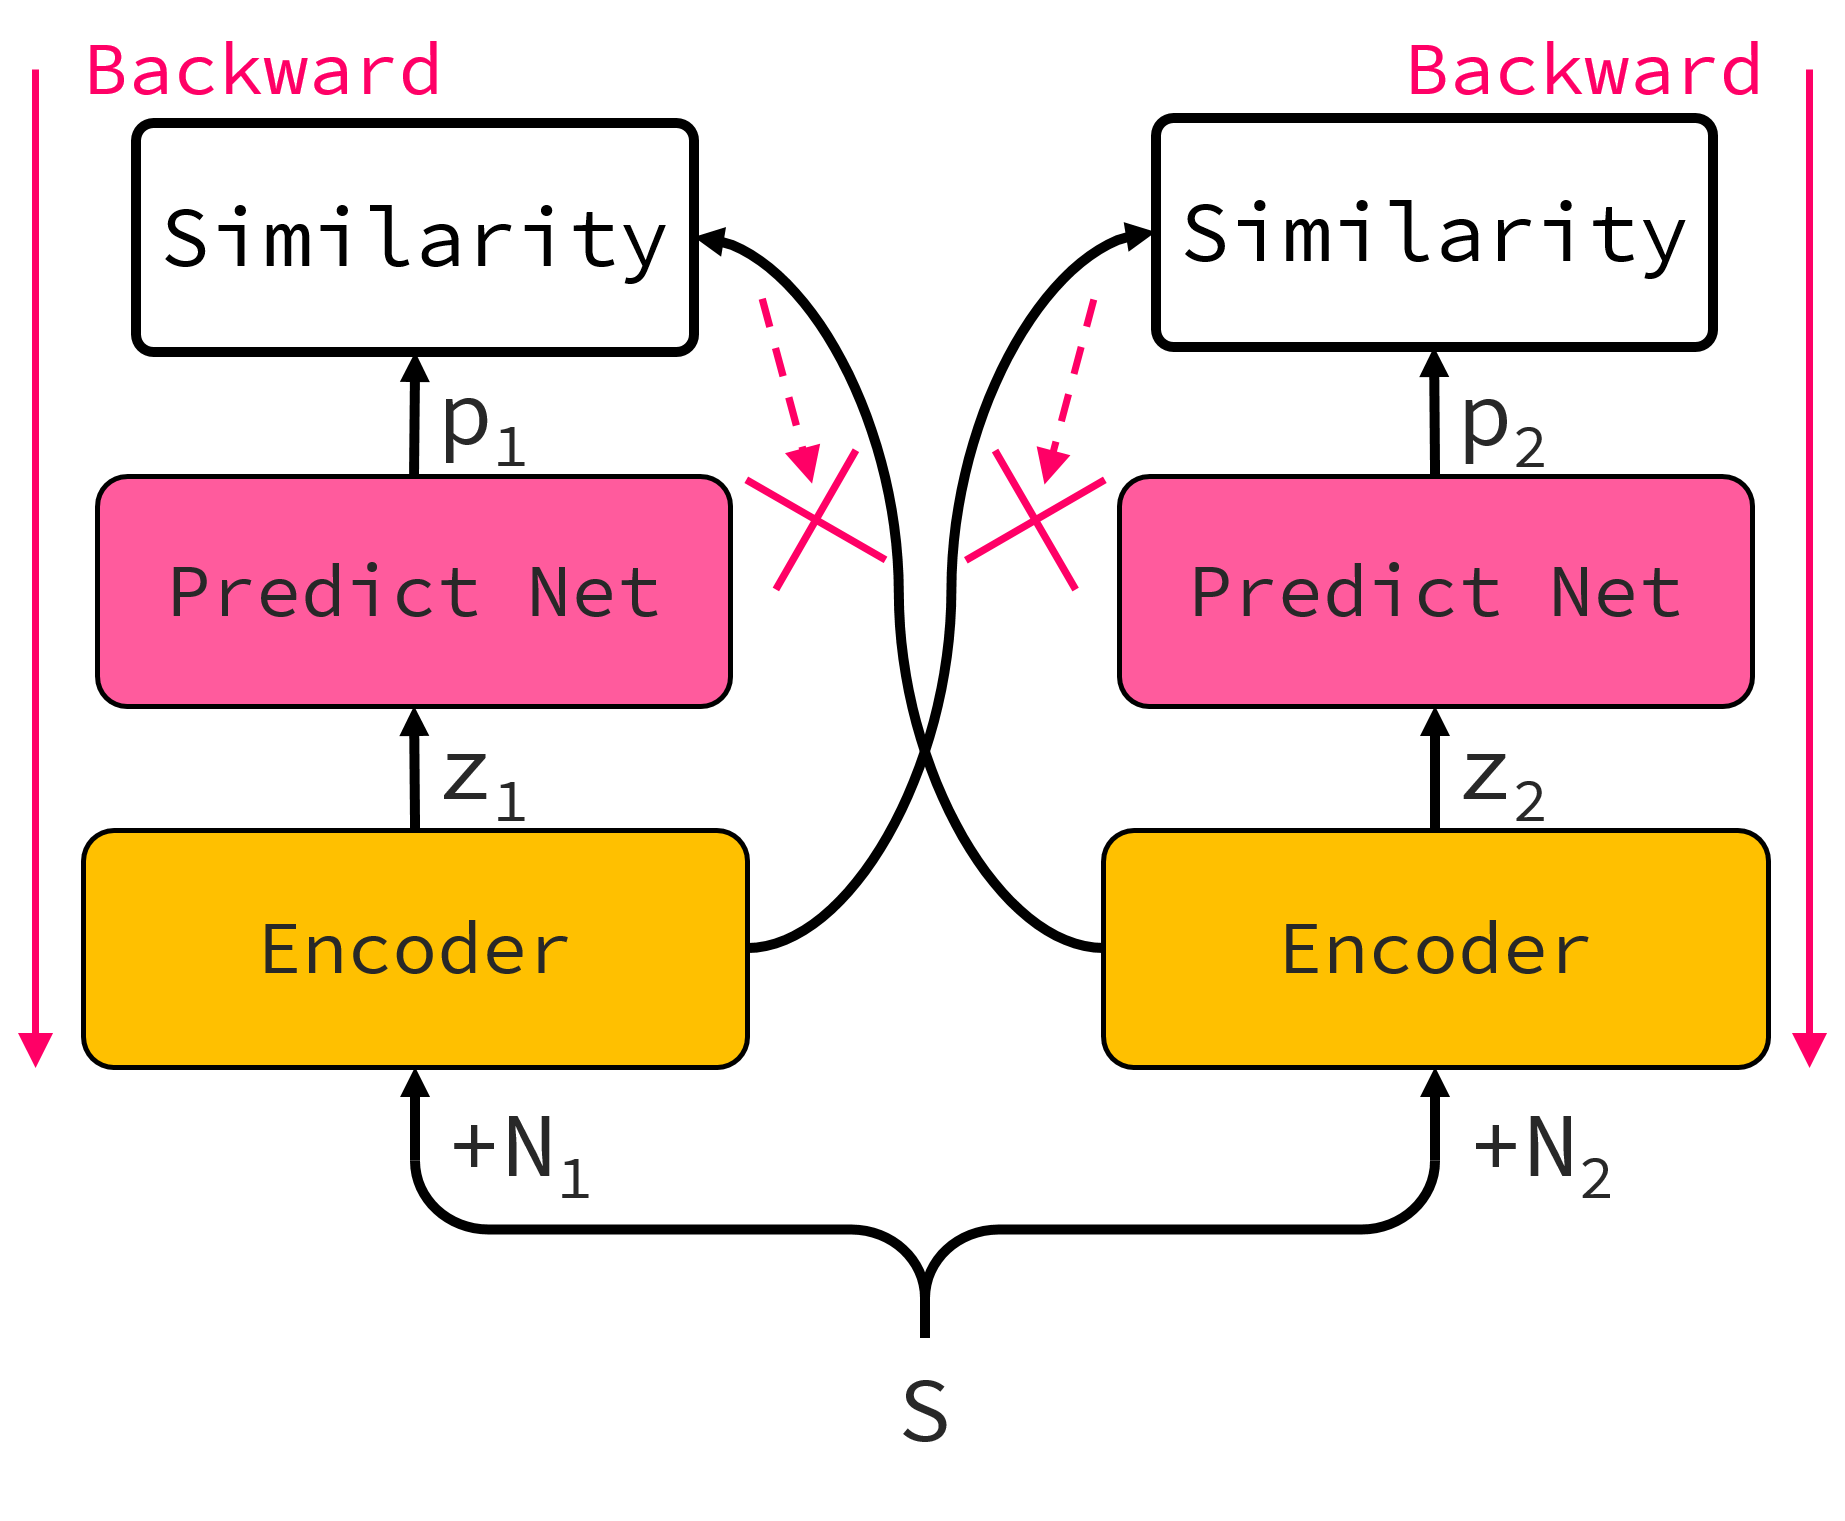
\includegraphics[width=1\linewidth]{img/SimSiam.png}
      \end{center}
      \caption{SimSiam 的算法架構。將混合不同噪音的語音輸入 Encoder 得到 $Z_1$ 與 $Z_2$,
         在將 $Z_1$ 與 $Z_2$ 輸入 PredictNet 後獲得 $P_1$ 與 $P_2$,
         $P_1$ 與 $P_2$ 會各自將 $Z_2$ 與 $Z_1$ 做為目標並計算差距,
         以此更新 Encoder-PredictNet 的參數。\label{fig:SimSiam}}
   \end{figure}
   %------------------------------------------------------------------------
   \section{Related works}
   Table.\ref{table:CL-methods} 對幾種常見的 Contrastive Learning 方法進行比較。包含 SimCLR~\cite{SimCLR} 在內的多數
   CL 方法都需要使用到大量的負樣本輔助進行訓練,否則會發生 collapsing output
   的問題,也就是不論輸入任何東西都只會有相同輸出。而大量的負樣本需求導致這些方法必須使用極大的 batch size 才能獲得良好效果,例如在
   SimCLR 的論文中,實驗所使用的 batch size 就到達了 4096。此外,Speech Enhancement 問題本身亦並不容易訂定 Frame Level
   的負樣本。為了因應硬體資源與 SE 任務的限制,本次研究使用 BYOL\cite{BYOL} 與 SimSiam\cite{SimSiam} 這兩項不需要極大 Batch Size,同時也不需負樣本的 Contrastive Learning 架構。

   \subsection{BYOL}
   BYOL 的架構流程如 Fig.\ref{fig:BYOL},模型主要可區分成 Encoder、Encoder$^{'}$ 與 Predictor
   這三大區塊,參數最佳化的目標即為 Predictor 輸出的特徵向量 p 與 Encoder$^{'}$ 輸出的特徵向量 z$^{'}$
   相似度越高越好:
   \begin{equation}
      Loss_{CL} = -\frac{Sim(p_1, sg(z^{'}_2))+Sim(p_2, sg(z^{'}_1))}{2}
      \label{eq:BYOL-Loss}
   \end{equation}
   Eq.\ref{eq:BYOL-Loss} 中的 sg 代表 stop gradient,因此在反傳遞過後,只有 Encoder 與 Predictor 會依靠梯度對參數進行更新,而 Encoder$^{'}$ 則是以 Momentum 的方式更新自身權重:
   \begin{equation}
      \theta_{E^{'}}=\tau\theta_{E^{'}}+(1-\tau)\theta_{E}
      \label{eq:Momentum}
   \end{equation}
   Eq.\ref{eq:Momentum} 中的 $\theta_{E^{'}}$ 與 $\theta_{E}$ 分別表示 Encoder$^{'}$ 與 Encoder 的參數。

   \subsection{SimSiam}
   SimSiam 與 BYOL 最大的差異是移除了 Momentum Encoder,除此之外的流程如 Fig.\ref{fig:SimSiam} 所示皆與 BYOL 相同:
   \begin{equation}
      Loss_{CL} = -\frac{Sim(p_1, sg(z_2))+Sim(p_2, sg(z_1))}{2}
      \label{eq:SimSiam-Loss}
   \end{equation}

   \begin{table}
      \caption{Contrastive Learning 方法比較。\label{table:CL-methods}}
      \begin{center}
         \begin{tabular}{ m{1.7cm} m{1.7cm} m{1.7cm} m{1.7cm} }
            CL Method        & Batch Size    & Negative Pairs     & Momentum Encoder \\
            \hline
            SimCLR           & 4096          & $\surd$            & $\times$         \\
            \hline
            MoCo v2          & 256           & $\surd$            & $\surd$          \\
            \hline
            \textbf{BYOL}    & 256$\sim$4096 & \textbf{$\times$}  & $\surd$          \\
            \hline
            SwAV             & 4096          & $\times$           & $\times$         \\
            \hline
            \textbf{SimSiam} & 256           & \textbf{$\times$ } & $\times$         \\
            \hline
         \end{tabular}
      \end{center}
   \end{table}

   %------------------------------------------------------------------------
   \section{Method}
   本專題使用的模型結構如 Figure 1. 所示,是由 Encoder 與 Decoder 兩區塊組合而成,
   其中負責抽取語音特徵 Encoder 區塊將會使用 BYOL 與 SimSiam 進行預訓練。
   在進行 CL 訓練時,語音 $S$ 會混合 $N_1$ 與 $N_2$ 兩個不同的噪音後,輸入 Encoder
   取出語音的特徵向量,並用 Figure 2. 與 Figure 3. 所述的方法更新其內部權重\footnote{在
      Figure 2. 與 Figure 3. 中的 X 符號代表 Stop Gradient,因此梯度並不會通過該區段向前更新。}。

   在使用 CL 預訓練完 Encoder 後,便會將其串接上
   Decoder,將乾淨的語音當成目標來進行語音增強任務的學習。更詳細的實驗內容在 Expected results 中。


   %------------------------------------------------------------------------
   \section{Experiments}
   本專題使用的噪音資料集是由 20 種不同類型的背景噪音所組成,總共有 100 個音檔的 Nonspeech~\cite{Nonspeech}。
   而語音資料集則是選用 TIMIT~\cite{TIMIT},TIMIT 具有 6300 句語音,這些語音包含美國八個地區共 630 人所念出的 10
   個指定句子。

   在訓練時的噪聲語音是將 4120 句 TIMIT 語音與 75 個 Nonspeech 雜訊以 -10, -5, 0, 5, 10 這三種 SNR
   混合產生的,其取樣頻率為 16K Hz,擷取時間約為 1s (16384 個樣本點)。測試則分別使用 500 與 25 個語音及噪音以 -7.5,
   -2.5, 2.5, 7.5 SNR 進行混合,並擷取約 2s (32768 個樣本點) 進行測試並計算其 PESQ\cite{PESQ}、STOI\cite{STOI} 及 SISDR\cite{SISDR}
   作為效能評估指標。

   實驗中訓練了使用 BYOL、SimSiam 以及未使用 CL 的 Normal 這大三類模型,並依據訓練過程中的 Loss
   切換方式,可區分為從頭到尾皆使用 Mix Loss 的基本模型,每 50 個 epoch 就在 Mix 與 SE Loss 之間切換的
   Round,與只有初期 50 個 epoch 使用 Mix Loss 後都使用 SE Loss 的 Pretrain。

   在 Fig.\ref{chart:CL-vs-Normal} 中比較 CL 方法的基本模型與 Normal 的收斂差異,BYOL 與 SimSiam
   在初期就以極快的速度提升效能。在 Fig.\ref{chart:BYOL-SimSiam} 則顯示基本模型與切換 Loss 的方法差異,不論
   BYOL 或是 SimSiam 皆呈現出在中期切換 Loss 可以加快模型收斂速度,但 SimSiam pretrain 在訓練後期明顯出現
   Overfitting 的問題,這代表在後期繼續使用 CL Loss 進行一定程度的約束是有必要的。

   為了測試 Contrastive Learning 在資料量不足情況是否也能夠提升模型效能,在 Fig.\ref{chart:few-data}
   的實驗中將測試資料與訓練資料互換,BYOL 與 SimSiam 的實驗結果依舊具備比 Normal 更優秀的表現。這表示即使只有少量資料,Contrastive
   Learning 依然能快速找出比一般方法更好的特徵。

   Table.\ref{table:Metrics} 記載了不同模型在三種評估指標下的結果。與 Normal 相比,所有使用了 CL
   的方法皆有明顯的效能提升。而不全程使用 CL Loss 約束的 Round 模型,則具備著比基礎模型更優秀的評估結果。在不同 SNR
   噪音下的表現,分別記錄在 Table.\ref{table:PESQ}、Table.\ref{table:STOI} 與 Table.\ref{table:SI-SDR}。

   \begin{figure}
      \begin{center}
         \begin{tikzpicture}
            \begin{axis}[
                  xlabel={epoch},
                  ylabel={Test SI-SNR},
                  ymin=0, ymax=10,
                  legend pos=south east,
                  mark=none,
                  ymajorgrids=true,
                  grid style=dashed,
                  legend entries={BYOL,SimSiam,Normal},
                  height = 6cm,
                  width = 9cm,
                  cycle list name=exotic,
               ]
               \addlegendimage{no markers, teal, line width=1pt}
               \addlegendimage{no markers, magenta, line width=1pt}
               \addlegendimage{no markers, cyan, line width=1pt}
               \addplot[mark=none, line width=0.5pt, color=teal] table [x=epoch, y=Test SISNR, col sep=comma] {../experiment/BYOL/history.csv};
               \addplot[mark=none, line width=0.5pt, color=magenta] table [x=epoch, y=Test SISNR, col sep=comma] {../experiment/SimSiam/history.csv};
               \addplot[mark=none, line width=0.5pt, color=cyan] table [x=epoch, y=Test SISNR, col sep=comma ] {../experiment/Normal/history.csv};
            \end{axis}
         \end{tikzpicture}
      \end{center}
      \caption{使用 BYOL、SimSiam 的模型與未使用 Contrastive Learning 方法的 Normal
         進行比較。可以發現 Contrastive Learning 在前期可以快速的提升模型的效能。\label{chart:CL-vs-Normal}}
   \end{figure}

   \begin{figure*}
      \begin{center}
         \begin{tikzpicture}
            \begin{axis}[
                  xlabel={epoch},
                  ylabel={Test SI-SNR},
                  ymin=0, ymax=10,
                  legend pos=south east,
                  mark=none,
                  ymajorgrids=true,
                  grid style=dashed,
                  legend entries={BYOL,BYOL round,BYOL round (100 step)},
                  height = 6cm,
                  width = 9cm,
                  cycle list name=exotic,
               ]
               \addlegendimage{no markers, teal, line width=1pt}
               \addlegendimage{no markers, magenta, line width=1pt}
               \addlegendimage{no markers, cyan, line width=1pt}
               \addplot[mark=none, line width=0.5pt, color=teal] table [x=epoch, y=Test SISNR, col sep=comma] {../experiment/BYOL/history.csv};
               \addplot[mark=none, line width=0.5pt, color=magenta] table [x=epoch, y=Test SISNR, col sep=comma] {../experiment/BYOL-round/history.csv};
               \addplot[mark=none, line width=0.5pt, color=cyan] table [x=epoch, y=Test SISNR, col sep=comma ] {../experiment/BYOL-round-100-step/history.csv};
            \end{axis}
         \end{tikzpicture}
         \begin{tikzpicture}
            \begin{axis}[
                  xlabel={epoch},
                  ylabel={Test SI-SNR},
                  ymin=0, ymax=10,
                  legend pos=south east,
                  mark=none,
                  ymajorgrids=true,
                  grid style=dashed,
                  legend entries={SimSiam,SimSiam round,SimSiam pretrain},
                  height = 6cm,
                  width = 9cm,
                  cycle list name=exotic,
               ]
               \addlegendimage{no markers, teal, line width=1pt}
               \addlegendimage{no markers, magenta, line width=1pt}
               \addlegendimage{no markers, cyan, line width=1pt}
               \addplot[mark=none, line width=0.5pt, color=teal] table [x=epoch, y=Test SISNR, col sep=comma] {../experiment/SimSiam/history.csv};
               \addplot[mark=none, line width=0.5pt, color=magenta] table [x=epoch, y=Test SISNR, col sep=comma] {../experiment/SimSiam-round/history.csv};
               \addplot[mark=none, line width=0.5pt, color=cyan] table [x=epoch, y=Test SISNR, col sep=comma ] {../experiment/SimSiam-pretrain/history.csv};
            \end{axis}
         \end{tikzpicture}
      \end{center}
      \caption{BYOL 與 SimSiam 的實驗結果。若在中後期減少 CL Loss 的約束力,反而能使模型效能提升更加迅速。但也可從
         SimSiam pretrain 的實驗也觀察到,若完全移除 CL Loss 會導致模型發生 overfitting。\label{chart:BYOL-SimSiam}}
   \end{figure*}


   \begin{figure}
      \begin{center}
         \begin{tikzpicture}
            \begin{axis}[
                  xlabel={epoch},
                  ylabel={Test SI-SNR},
                  ymin=0, ymax=6,
                  legend pos=south east,
                  mark=none,
                  ymajorgrids=true,
                  grid style=dashed,
                  legend entries={BYOL few,SimSiam few,Normal few},
                  height = 6cm,
                  width = 9cm,
                  cycle list name=exotic,
               ]
               \addlegendimage{no markers, teal, line width=1pt}
               \addlegendimage{no markers, magenta, line width=1pt}
               \addlegendimage{no markers, cyan, line width=1pt}
               \addplot[mark=none, line width=0.5pt, color=teal] table [x=epoch, y=Test SISNR, col sep=comma] {../experiment/BYOL-few/history.csv};
               \addplot[mark=none, line width=0.5pt, color=magenta] table [x=epoch, y=Test SISNR, col sep=comma] {../experiment/SimSiam-few/history.csv};
               \addplot[mark=none, line width=0.5pt, color=cyan] table [x=epoch, y=Test SISNR, col sep=comma ] {../experiment/Normal-few/history.csv};
            \end{axis}
         \end{tikzpicture}
      \end{center}
      \caption{改為使用測試集進行訓練、訓練集進行測試。即使是在只有少量資料的情況,Contrastive Learning
         依然比只使用 Speech Enhancement Loss 的方法具有更高的效能。\label{chart:few-data}}
   \end{figure}


   \begin{table}
      \caption{各模型的對噪聲語音進行去噪後的平均評估結果\label{table:Metrics}}
      \begin{center}
         \begin{tabular}{ l c c c  }
            \multirow{2}{4em}{Model}   & \multicolumn{3}{ c } {Evaluation Metrics}                                   \\
            \cline{2-4}
                                       & PESQ                                      & STOI           & SI-SNR         \\
            \hline
            Noisy                      & 1.813                                     & 0.764          & 0.001          \\
            \hline
            Normal                     & 2.273                                     & 0.814          & 7.146          \\
            \hline
            BYOL                       & 2.392                                     & 0.844          & 9.174          \\
            \hline
            BYOL round                 & 2.461                                     & 0.858          & 9.378          \\
            \hline
            \textbf{BYOL round(100 s)} & \textbf{2.474}                            & \textbf{0.861} & \textbf{9.526} \\
            \hline
            SimSiam                    & 2.374                                     & 0.84           & 8.884          \\
            \hline
            \textbf{SimSiam round}     & \textbf{2.472}                            & \textbf{0.861} & \textbf{9.529} \\
            \hline
         \end{tabular}
      \end{center}
   \end{table}

   \begin{table}
      \caption{各模型的對混和不同 SNR 雜訊進行去噪後的 PESQ 評估結果\label{table:PESQ}}
      \begin{center}
         \begin{tabular}{ l c c c c  }
            \multirow{2}{4em}{Model}   & -7.5                        & -2.5           & 2.5            & 7.5            \\
            \cline{2-5}
                                       & \multicolumn{4}{ c } {PESQ}                                                    \\
            \hline
            Noisy                      & 1.337                       & 1.644          & 1.971          & 2.3            \\
            \hline
            Normal                     & 1.826                       & 2.138          & 2.438          & 2.688          \\
            \hline
            BYOL                       & 1.875                       & 2.253          & 2.59           & 2.851          \\
            \hline
            BYOL round                 & 1.904                       & 2.3            & 2.671          & 2.97           \\
            \hline
            \textbf{BYOL round(100 s)} & \textbf{1.913}              & \textbf{2.308} & \textbf{2.683} & \textbf{2.991} \\
            \hline
            SimSiam                    & 1.873                       & 2.24           & 2.563          & 2.82           \\
            \hline
            \textbf{SimSiam round}     & \textbf{1.937}              & \textbf{2.317} & \textbf{2.672} & \textbf{2.962} \\
            \hline
         \end{tabular}
      \end{center}
   \end{table}


   \begin{table}
      \caption{各模型的對混和不同 SNR 雜訊進行去噪後的 STOI 評估結果\label{table:STOI}}
      \begin{center}
         \begin{tabular}{ l c c c  c}
            \multirow{2}{4em}{Model}   & -7.5                        & -2.5           & 2.5            & 7.5            \\
            \cline{2-5}
                                       & \multicolumn{4}{ c } {STOI}                                                    \\
            \hline
            Noisy                      & 0.643                       & 0.728          & 0.809          & 0.878          \\
            \hline
            Normal                     & 0.702                       & 0.793          & 0.859          & 0.904          \\
            \hline
            BYOL                       & 0.734                       & 0.826          & 0.889          & 0.928          \\
            \hline
            BYOL round                 & 0.746                       & 0.841          & 0.904          & 0.942          \\
            \hline
            \textbf{BYOL round(100 s)} & \textbf{0.75}               & \textbf{0.844} & \textbf{0.906} & \textbf{0.944} \\
            \hline
            SimSiam                    & 0.729                       & 0.822          & 0.885          & 0.926          \\
            \hline
            \textbf{SimSiam round}     & \textbf{0.753}              & \textbf{0.845} & \textbf{0.905} & \textbf{0.942} \\
            \hline
         \end{tabular}
      \end{center}
   \end{table}

   \begin{table}
      \caption{各模型的對混和不同 SNR 雜訊進行去噪後的 SI-SDR 評估結果\label{table:SI-SDR}}
      \begin{center}
         \begin{tabular}{ l c c c c }
            \multirow{2}{4em}{Model}   & -7.5                          & -2.5           & 2.5             & 7.5             \\
            \cline{2-5}
                                       & \multicolumn{4}{ c } {SI-SDR}                                                      \\
            \hline
            Noisy                      & -7.497                        & -2.498         & 2.503           & 7.498           \\
            \hline
            Normal                     & 2.611                         & 6.065          & 8.972           & 10.935          \\
            \hline
            BYOL                       & 3.677                         & 7.785          & 11.281          & 13.951          \\
            \hline
            BYOL round                 & 3.396                         & 7.772          & 11.615          & 14.728          \\
            \hline
            \textbf{BYOL round(100 s)} & \textbf{3.457}                & \textbf{7.859} & \textbf{11.784} & \textbf{15.004} \\
            \hline
            SimSiam                    & 3.544                         & 7.508          & 10.913          & 13.572          \\
            \hline
            \textbf{SimSiam round}     & \textbf{3.583}                & \textbf{7.935} & \textbf{11.751} & \textbf{14.847} \\
            \hline
         \end{tabular}
      \end{center}
   \end{table}
   %------------------------------------------------------------------------
   \section{Conclusion}
   本次將 Contrastive Learning 運用於 Speech Enhancement 的研究結果可發現,前期使用 CL Loss
   對中間的隱藏特徵進行高強度的約束,能提升模型的收斂速度。然而若在中後期繼續讓 CL Loss
   維持較高的權重反而會阻礙模型提升效能。但這並不代表 CL Loss 就完全不重要,相反的,保持一定程度的
   CL 約束能有效避免 Overfitting 的發生。

   未來將使用兩種以上的雜訊與語音進行混和,以驗證在更加複雜的資料擴增下使用 Contrastive
   Learning,能否讓 Speech Enhancement 的效能有更大幅度的提升。並研究具有自適應性的
   CL Loss 與 SE Loss 權重調整方法,好減少人工調整超參數的麻煩。

   {\small
   \bibliographystyle{ieee_fullname}
   \bibliography{egbib}
   }
\end{CJK}
\end{document}
